% =============================================================================
%  Reporte técnico (formato APA 7.ª ed.) - MongoDB frente a PostgreSQL JSONB
%  bajo límites de recursos de cgroups v2.
%
%  Compilar (sin biber; la lista de referencias es manual):
%      pdflatex reporte_tecnico.tex   (dos pasadas)
%  Regenerar figuras, tablas y cifras desde los resultados reales:
%      ./.venv/Scripts/python.exe report/src/build_assets.py
%
%  EDITAR: los datos de la portada (autor, docente, fecha) están en el bloque
%  "DATOS DE LA PORTADA" justo debajo.
% =============================================================================
\documentclass[12pt,letterpaper]{article}

\usepackage[utf8]{inputenc}
\usepackage[T1]{fontenc}
\usepackage{mathptmx}                 % Times (estilo APA)
\usepackage[spanish]{babel}
\usepackage[margin=1in]{geometry}
\usepackage{amsmath}
\usepackage{setspace}
\usepackage{graphicx}
\usepackage{booktabs}
\usepackage{longtable}
\usepackage{array}
\usepackage{caption}
\usepackage{placeins}
\usepackage{fancyhdr}
\usepackage{titlesec}
\usepackage{verbatim}
\usepackage{url}
\usepackage[hidelinks,breaklinks]{hyperref}

\addto\captionsspanish{\renewcommand{\tablename}{Tabla}\renewcommand{\figurename}{Figura}}
\AtBeginDocument{\shorthandoff{<>}}

% ---------------------------------------------------------------- DATOS DE LA PORTADA
\newcommand{\autor}{[Nombre del autor]}
\newcommand{\docente}{[Nombre del docente]}
\newcommand{\fechaentrega}{1 de noviembre de 2026}
\newcommand{\institucion}{Universidad Politécnica de Chiapas}
\newcommand{\programa}{Ingeniería en Tecnologías de la Información e Innovación Digital (IT2iD)}
\newcommand{\curso}{Bases de Datos en la Nube}
\newcommand{\titulo}{Contención de CPU y memoria en agregaciones JSON: evaluación experimental de MongoDB 9.0.4 frente a PostgreSQL 18.6 JSONB bajo cgroups v2}

% cifras calculadas a partir de results/ (generadas por build_assets.py)
\newcommand{\defFact}[2]{\expandafter\def\csname fact@#1\endcsname{#2}}
\newcommand{\fact}[1]{\csname fact@#1\endcsname}
\defFact{Q1Ac10mp99}{8\,723}
\defFact{Q1Ac10mqps}{1.38}
\defFact{Q1Ac10mthr}{2}
\defFact{Q1Ac10pp99}{83\,191}
\defFact{Q1Ac10pqps}{0.19}
\defFact{Q1Ac10pthr}{0}
\defFact{Q1Ac10rcpu}{3.1}
\defFact{Q1Ac10rmem}{12.6}
\defFact{Q1Ac10rp99}{9.5}
\defFact{Q1Ac10rqps}{7.2}
\defFact{Q1Ac10rqpsinv}{0.1}
\defFact{Q1Ac1mp99}{1\,949}
\defFact{Q1Ac1mqps}{0.65}
\defFact{Q1Ac1mthr}{0}
\defFact{Q1Ac1pp99}{7\,967}
\defFact{Q1Ac1pqps}{0.33}
\defFact{Q1Ac1pthr}{0}
\defFact{Q1Ac1rcpu}{3.2}
\defFact{Q1Ac1rmem}{1.8}
\defFact{Q1Ac1rp99}{4.1}
\defFact{Q1Ac1rqps}{1.9}
\defFact{Q1Ac1rqpsinv}{0.5}
\defFact{Q1Ac50mp99}{42\,502}
\defFact{Q1Ac50mqps}{1.33}
\defFact{Q1Ac50mthr}{3}
\defFact{Q1Ac50pp99}{204\,550}
\defFact{Q1Ac50pqps}{0.18}
\defFact{Q1Ac50pthr}{0}
\defFact{Q1Ac50rcpu}{3.8}
\defFact{Q1Ac50rmem}{20.0}
\defFact{Q1Ac50rp99}{4.8}
\defFact{Q1Ac50rqps}{7.4}
\defFact{Q1Ac50rqpsinv}{0.1}
\defFact{Q1Bc10mp99}{14\,802}
\defFact{Q1Bc10mqps}{0.85}
\defFact{Q1Bc10mthr}{597}
\defFact{Q1Bc10pp99}{59\,291}
\defFact{Q1Bc10pqps}{0.19}
\defFact{Q1Bc10pthr}{446}
\defFact{Q1Bc10rcpu}{4.3}
\defFact{Q1Bc10rmem}{6.9}
\defFact{Q1Bc10rp99}{4.0}
\defFact{Q1Bc10rqps}{4.4}
\defFact{Q1Bc10rqpsinv}{0.2}
\defFact{Q1Bc1mp99}{2\,149}
\defFact{Q1Bc1mqps}{0.61}
\defFact{Q1Bc1mthr}{0}
\defFact{Q1Bc1pp99}{3\,822}
\defFact{Q1Bc1pqps}{0.30}
\defFact{Q1Bc1pthr}{103}
\defFact{Q1Bc1rcpu}{2.9}
\defFact{Q1Bc1rmem}{1.7}
\defFact{Q1Bc1rp99}{1.8}
\defFact{Q1Bc1rqps}{2.0}
\defFact{Q1Bc1rqpsinv}{0.5}
\defFact{Q1Bc50mp99}{63\,186}
\defFact{Q1Bc50mqps}{0.86}
\defFact{Q1Bc50mthr}{595}
\defFact{Q1Bc50pp99}{---}
\defFact{Q1Bc50pqps}{0.00}
\defFact{Q1Bc50pthr}{424}
\defFact{Q1Cc10mp99}{31\,353}
\defFact{Q1Cc10mqps}{0.40}
\defFact{Q1Cc10mthr}{894}
\defFact{Q1Cc10pp99}{146\,758}
\defFact{Q1Cc10pqps}{0.09}
\defFact{Q1Cc10pthr}{740}
\defFact{Q1Cc10rcpu}{4.3}
\defFact{Q1Cc10rmem}{8.3}
\defFact{Q1Cc10rp99}{4.7}
\defFact{Q1Cc10rqps}{4.5}
\defFact{Q1Cc10rqpsinv}{0.2}
\defFact{Q1Cc1mp99}{2\,598}
\defFact{Q1Cc1mqps}{0.52}
\defFact{Q1Cc1mthr}{12}
\defFact{Q1Cc1pp99}{8\,279}
\defFact{Q1Cc1pqps}{0.14}
\defFact{Q1Cc1pthr}{219}
\defFact{Q1Cc1rcpu}{3.5}
\defFact{Q1Cc1rmem}{2.1}
\defFact{Q1Cc1rp99}{3.2}
\defFact{Q1Cc1rqps}{3.6}
\defFact{Q1Cc1rqpsinv}{0.3}
\defFact{Q1Cc50mp99}{127\,111}
\defFact{Q1Cc50mqps}{0.50}
\defFact{Q1Cc50mthr}{893}
\defFact{Q1Cc50pp99}{---}
\defFact{Q1Cc50pqps}{0.00}
\defFact{Q1Cc50pthr}{787}
\defFact{Q2Ac10mp99}{2\,844}
\defFact{Q2Ac10mqps}{4.94}
\defFact{Q2Ac10mthr}{2}
\defFact{Q2Ac10pp99}{3\,420}
\defFact{Q2Ac10pqps}{4.95}
\defFact{Q2Ac10pthr}{1}
\defFact{Q2Ac10rcpu}{1.0}
\defFact{Q2Ac10rmem}{1.4}
\defFact{Q2Ac10rp99}{1.2}
\defFact{Q2Ac10rqps}{1.0}
\defFact{Q2Ac10rqpsinv}{1.0}
\defFact{Q2Ac1mp99}{715}
\defFact{Q2Ac1mqps}{1.87}
\defFact{Q2Ac1mthr}{0}
\defFact{Q2Ac1pp99}{291}
\defFact{Q2Ac1pqps}{4.01}
\defFact{Q2Ac1pthr}{0}
\defFact{Q2Ac1rcpu}{1.3}
\defFact{Q2Ac1rmem}{0.6}
\defFact{Q2Ac1rp99}{0.4}
\defFact{Q2Ac1rqps}{0.5}
\defFact{Q2Ac1rqpsinv}{2.1}
\defFact{Q2Ac50mp99}{11\,526}
\defFact{Q2Ac50mqps}{4.75}
\defFact{Q2Ac50mthr}{2}
\defFact{Q2Ac50pp99}{11\,552}
\defFact{Q2Ac50pqps}{5.47}
\defFact{Q2Ac50pthr}{1}
\defFact{Q2Ac50rcpu}{0.9}
\defFact{Q2Ac50rmem}{1.5}
\defFact{Q2Ac50rp99}{1.0}
\defFact{Q2Ac50rqps}{0.9}
\defFact{Q2Ac50rqpsinv}{1.2}
\defFact{Q2Bc10mp99}{16\,982}
\defFact{Q2Bc10mqps}{0.77}
\defFact{Q2Bc10mthr}{585}
\defFact{Q2Bc10pp99}{7\,657}
\defFact{Q2Bc10pqps}{2.22}
\defFact{Q2Bc10pthr}{540}
\defFact{Q2Bc10rcpu}{0.3}
\defFact{Q2Bc10rmem}{0.4}
\defFact{Q2Bc10rp99}{0.5}
\defFact{Q2Bc10rqps}{0.3}
\defFact{Q2Bc10rqpsinv}{2.9}
\defFact{Q2Bc1mp99}{3\,239}
\defFact{Q2Bc1mqps}{0.39}
\defFact{Q2Bc1mthr}{0}
\defFact{Q2Bc1pp99}{567}
\defFact{Q2Bc1pqps}{2.69}
\defFact{Q2Bc1pthr}{316}
\defFact{Q2Bc1rcpu}{0.3}
\defFact{Q2Bc1rmem}{0.1}
\defFact{Q2Bc1rp99}{0.2}
\defFact{Q2Bc1rqps}{0.1}
\defFact{Q2Bc1rqpsinv}{6.9}
\defFact{Q2Bc50mp99}{98\,309}
\defFact{Q2Bc50mqps}{0.65}
\defFact{Q2Bc50mthr}{594}
\defFact{Q2Bc50pp99}{30\,744}
\defFact{Q2Bc50pqps}{2.79}
\defFact{Q2Bc50pthr}{583}
\defFact{Q2Bc50rcpu}{0.2}
\defFact{Q2Bc50rmem}{0.4}
\defFact{Q2Bc50rp99}{0.3}
\defFact{Q2Bc50rqps}{0.2}
\defFact{Q2Bc50rqpsinv}{4.3}
\defFact{Q2Cc10mp99}{55\,053}
\defFact{Q2Cc10mqps}{0.33}
\defFact{Q2Cc10mthr}{821}
\defFact{Q2Cc10pp99}{21\,961}
\defFact{Q2Cc10pqps}{0.77}
\defFact{Q2Cc10pthr}{643}
\defFact{Q2Cc10rcpu}{0.4}
\defFact{Q2Cc10rmem}{0.5}
\defFact{Q2Cc10rp99}{0.4}
\defFact{Q2Cc10rqps}{0.4}
\defFact{Q2Cc10rqpsinv}{2.3}
\defFact{Q2Cc1mp99}{6\,530}
\defFact{Q2Cc1mqps}{0.18}
\defFact{Q2Cc1mthr}{17}
\defFact{Q2Cc1pp99}{1\,093}
\defFact{Q2Cc1pqps}{1.18}
\defFact{Q2Cc1pthr}{552}
\defFact{Q2Cc1rcpu}{0.1}
\defFact{Q2Cc1rmem}{0.1}
\defFact{Q2Cc1rp99}{0.2}
\defFact{Q2Cc1rqps}{0.2}
\defFact{Q2Cc1rqpsinv}{6.6}
\defFact{Q2Cc50mp99}{334\,436}
\defFact{Q2Cc50mqps}{0.17}
\defFact{Q2Cc50mthr}{883}
\defFact{Q2Cc50pp99}{196\,714}
\defFact{Q2Cc50pqps}{0.54}
\defFact{Q2Cc50pthr}{717}
\defFact{Q2Cc50rcpu}{0.3}
\defFact{Q2Cc50rmem}{0.6}
\defFact{Q2Cc50rp99}{0.6}
\defFact{Q2Cc50rqps}{0.3}
\defFact{Q2Cc50rqpsinv}{3.3}
\defFact{annexok}{63}
\defFact{annexoom}{6}
\defFact{annexspill}{3}
\defFact{annextotal}{72}
\defFact{discarded}{31}
\defFact{dpQ1mBc1}{10}
\defFact{dpQ1mBc10}{70}
\defFact{dpQ1mBc50}{49}
\defFact{dpQ1mCc1}{33}
\defFact{dpQ1mCc10}{259}
\defFact{dpQ1mCc50}{199}
\defFact{dpQ1pBc1}{-52}
\defFact{dpQ1pBc10}{-29}
\defFact{dpQ1pCc1}{4}
\defFact{dpQ1pCc10}{76}
\defFact{dpQ2mBc1}{353}
\defFact{dpQ2mBc10}{497}
\defFact{dpQ2mBc50}{753}
\defFact{dpQ2mCc1}{813}
\defFact{dpQ2mCc10}{1836}
\defFact{dpQ2mCc50}{2802}
\defFact{dpQ2pBc1}{95}
\defFact{dpQ2pBc10}{124}
\defFact{dpQ2pBc50}{166}
\defFact{dpQ2pCc1}{276}
\defFact{dpQ2pCc10}{542}
\defFact{dpQ2pCc50}{1603}
\defFact{dqQ1mBc1}{6}
\defFact{dqQ1mBc10}{39}
\defFact{dqQ1mBc50}{35}
\defFact{dqQ1mCc1}{20}
\defFact{dqQ1mCc10}{71}
\defFact{dqQ1mCc50}{62}
\defFact{dqQ1pBc1}{10}
\defFact{dqQ1pBc10}{0}
\defFact{dqQ1pBc50}{100}
\defFact{dqQ1pCc1}{57}
\defFact{dqQ1pCc10}{53}
\defFact{dqQ1pCc50}{100}
\defFact{dqQ2mBc1}{79}
\defFact{dqQ2mBc10}{84}
\defFact{dqQ2mBc50}{86}
\defFact{dqQ2mCc1}{91}
\defFact{dqQ2mCc10}{93}
\defFact{dqQ2mCc50}{96}
\defFact{dqQ2pBc1}{33}
\defFact{dqQ2pBc10}{55}
\defFact{dqQ2pBc50}{49}
\defFact{dqQ2pCc1}{71}
\defFact{dqQ2pCc10}{84}
\defFact{dqQ2pCc50}{90}
\defFact{finished}{180}
\defFact{halts}{3}
\defFact{hours}{36.7}
\defFact{incidents}{9}
\defFact{mainok}{81}
\defFact{mainoom}{6}
\defFact{mainspill}{21}
\defFact{maintotal}{108}
\defFact{oomkills}{580}
\defFact{oomrssmax}{1763}
\defFact{pgq1estrows}{16\,504\,191}
\defFact{planQ1Amgdocs}{500\,000}
\defFact{planQ1Amgkeys}{0}
\defFact{planQ1Amgms}{3\,221}
\defFact{planQ1Apgdisk}{705}
\defFact{planQ1Apgms}{5\,654}
\defFact{planQ1Cmgdocs}{500\,000}
\defFact{planQ1Cmgkeys}{0}
\defFact{planQ1Cmgms}{3\,482}
\defFact{planQ1Cpgdisk}{705}
\defFact{planQ1Cpgms}{8\,041}
\defFact{planQ2Amgdocs}{226\,680}
\defFact{planQ2Amgkeys}{226\,680}
\defFact{planQ2Amgms}{5\,591}
\defFact{planQ2Apgdisk}{0}
\defFact{planQ2Apgms}{2\,201}
\defFact{planQ2Cmgdocs}{226\,680}
\defFact{planQ2Cmgkeys}{226\,680}
\defFact{planQ2Cmgms}{9\,098}
\defFact{planQ2Cpgdisk}{0}
\defFact{planQ2Cpgms}{2\,561}
\defFact{relQ1mCc1}{0.76}
\defFact{relQ1mCc10}{0.80}
\defFact{relQ1mCc50}{0.89}
\defFact{relQ1pCc1}{0.73}
\defFact{relQ2mAc1}{1.02}
\defFact{relQ2mAc10}{1.01}
\defFact{relQ2mAc50}{1.06}
\defFact{relQ2mBc1}{1.03}
\defFact{relQ2mBc10}{1.10}
\defFact{relQ2mBc50}{1.00}
\defFact{relQ2mCc1}{0.87}
\defFact{relQ2mCc10}{0.49}
\defFact{relQ2mCc50}{0.90}
\defFact{relQ2pAc1}{1.06}
\defFact{relQ2pAc10}{0.99}
\defFact{relQ2pAc50}{0.97}
\defFact{relQ2pBc1}{0.89}
\defFact{relQ2pBc10}{0.99}
\defFact{relQ2pBc50}{0.93}
\defFact{relQ2pCc1}{0.91}
\defFact{relQ2pCc10}{0.98}
\defFact{relQ2pCc50}{0.95}
\defFact{relq2max}{1.10}
\defFact{relq2min}{0.49}
\defFact{relqQ1mCc1}{1.12}
\defFact{relqQ1mCc10}{1.21}
\defFact{relqQ1mCc50}{1.00}
\defFact{relqQ1pCc1}{1.24}
\defFact{relqQ2mAc1}{1.01}
\defFact{relqQ2mAc10}{0.94}
\defFact{relqQ2mAc50}{0.96}
\defFact{relqQ2mBc1}{0.98}
\defFact{relqQ2mBc10}{1.03}
\defFact{relqQ2mBc50}{0.98}
\defFact{relqQ2mCc1}{1.11}
\defFact{relqQ2mCc10}{1.20}
\defFact{relqQ2mCc50}{1.00}
\defFact{relqQ2pAc1}{0.98}
\defFact{relqQ2pAc10}{1.00}
\defFact{relqQ2pAc50}{0.99}
\defFact{relqQ2pBc1}{0.88}
\defFact{relqQ2pBc10}{1.05}
\defFact{relqQ2pBc50}{1.04}
\defFact{relqQ2pCc1}{1.10}
\defFact{relqQ2pCc10}{0.99}
\defFact{relqQ2pCc50}{0.99}
\defFact{resumes}{21}


% ---------------------------------------------------------------- formato APA
\setlength{\parindent}{0.5in}
\setlength{\parskip}{0pt}
\raggedright
\setcounter{secnumdepth}{0}
\pagestyle{fancy}
\fancyhf{}
\fancyhead[R]{\thepage}
\renewcommand{\headrulewidth}{0pt}
\setlength{\headheight}{15pt}

\titleformat{\section}{\normalfont\normalsize\bfseries\centering}{}{0pt}{}
\titleformat{\subsection}{\normalfont\normalsize\bfseries}{}{0pt}{}
\titleformat{\subsubsection}{\normalfont\normalsize\bfseries\itshape}{}{0pt}{}
\titlespacing*{\section}{0pt}{0pt}{0pt}
\titlespacing*{\subsection}{0pt}{0pt}{0pt}
\titlespacing*{\subsubsection}{0pt}{0pt}{0pt}

\captionsetup[table]{labelfont=bf,labelsep=newline,textfont=it,justification=raggedright,singlelinecheck=false,position=top,skip=4pt}
\captionsetup[figure]{labelfont=bf,labelsep=newline,textfont=it,justification=raggedright,singlelinecheck=false,position=top,skip=4pt}

\newenvironment{apatab}[1][!htbp]{\begin{table}[#1]\singlespacing}{\end{table}}
\newenvironment{apafig}[1][!htbp]{\begin{figure}[#1]\singlespacing}{\end{figure}}
\newcommand{\apanote}[1]{\par\vspace{3pt}{\footnotesize\noindent\textit{Nota.} #1\par}}
\newcommand{\aparef}[1]{\par\noindent\hangindent=0.5in\hangafter=1 #1\par}
\newcommand{\code}[1]{\texttt{#1}}
\newcommand{\tablefile}[1]{{\footnotesize\setlength{\tabcolsep}{3pt}\input{tables/#1}}}
\newcommand{\Mongo}{MongoDB}
\newcommand{\PG}{PostgreSQL}

\begin{document}
\doublespacing

% =============================================================================  PORTADA
\thispagestyle{fancy}
\begin{center}
\vspace*{1.2in}
{\bfseries \titulo\par}
\vspace{1\baselineskip}
\autor\par
\institucion\par
\programa\par
\curso\par
\docente\par
\fechaentrega\par
\end{center}
\clearpage

% =============================================================================  RESUMEN
\section{Resumen}
\noindent
Se evaluó experimentalmente cómo se comportan MongoDB 9.0.4 y PostgreSQL 18.6 (JSONB) al ejecutar dos
consultas analíticas sobre un corpus sintético de 500\,000 órdenes de comercio electrónico cuando el
contenedor que aloja al motor se restringe con límites de CPU y memoria de cgroups v2. Se midieron 180 corridas
(108 de la matriz principal y 72 de un anexo que contrasta la memoria estricta con la relajada) sobre tres
perfiles de recursos (4, 2 y 1 CPU con 4, 2 y 1 GiB de RAM), tres niveles de concurrencia (1, 10 y 50 clientes) y tres
repeticiones por celda, con latencias P50/P95/P99, rendimiento, tiempo de limitación de CFS, volcado a disco y
huella de recursos por cada 1\,000 documentos. En la agregación con desanidado de arreglos (Q1),
MongoDB obtuvo un rendimiento entre \fact{Q1Ac1rqps} y \fact{Q1Ac50rqps} veces mayor que PostgreSQL en el
perfil sin restricción, mientras que PostgreSQL volcó a disco en todas las corridas de Q1 y fue terminado por falta de memoria
con 50 clientes en los perfiles de 2 y 1 GiB. En la consulta con orden acotado (Q2), PostgreSQL fue
más eficiente bajo restricción (hasta \fact{Q2Bc1rqpsinv} veces el rendimiento de MongoDB con 2 CPU y un cliente), porque
recorre la tabla de forma secuencial, mientras que MongoDB accede a 226\,680 documentos por índice. Elevar \code{work\_mem} a 64 MB
no mitigó el volcado y adelantó el agotamiento de memoria con 10 clientes. Se documentan las limitaciones de la
medición y las recomendaciones de dimensionamiento para despliegues en la nube.

\vspace{0.5\baselineskip}
\noindent\hspace{0.5in}\textit{Palabras clave:} MongoDB, PostgreSQL, JSONB, cgroups v2, CFS, latencia de cola, benchmark
\clearpage

\section{Abstract}
\noindent
This report experimentally compares MongoDB 9.0.4 and PostgreSQL 18.6 (JSONB) running two analytical queries over a
synthetic corpus of 500,000 e-commerce orders while the database container is constrained with cgroups v2 CPU and
memory limits. A total of 180 runs (108 in the main matrix and 72 in a strict-versus-relaxed memory annex) were
collected across three resource profiles (4, 2, and 1 CPU with 4, 2, and 1 GiB of RAM), three concurrency levels
(1, 10, and 50 clients), and three repetitions per cell, recording P50/P95/P99 latency, throughput, CFS throttling time,
disk spills, and per-1,000-document resource footprint. For the array-unwinding aggregation (Q1), MongoDB delivered
\fact{Q1Ac1rqps} to \fact{Q1Ac50rqps} times the throughput of PostgreSQL in the unconstrained profile, while PostgreSQL
spilled to disk in every Q1 run and was killed by the out-of-memory killer at 50 clients in the 2 GiB and 1 GiB
profiles. For the bounded top-N query (Q2), PostgreSQL was more efficient under constraint because it scans sequentially,
whereas MongoDB fetched 226,680 documents through an index. Raising \code{work\_mem} to 64 MB did not prevent spilling and
anticipated memory exhaustion at 10 clients. Measurement limitations and sizing recommendations for cloud deployments are discussed.

\vspace{0.5\baselineskip}
\noindent\hspace{0.5in}\textit{Keywords:} MongoDB, PostgreSQL, JSONB, cgroups v2, CFS, tail latency, benchmark
\clearpage

% =============================================================================  CUERPO
\begin{center}\bfseries \titulo\end{center}

\section{Introducción}
Los motores documentales y los relacionales con soporte JSON compiten por las mismas cargas: almacenar documentos
anidados y consultarlos de forma analítica. En producción, ambos suelen ejecutarse dentro de contenedores
cuyos recursos están acotados por el orquestador mediante cuotas de CPU y límites de memoria
(Merkel, 2014; Heo, s.\,f.). Esa restricción cambia el problema: ya no basta con comparar el rendimiento de dos
motores con máquina completa, porque la cuota de CFS (\textit{Completely Fair Scheduler}) puede detener al contenedor
aunque haya CPU libre en el anfitrión, y el límite de memoria sin \textit{swap} convierte un exceso de uso en la
terminación del proceso. Además, la latencia de cola, y no el promedio, es la que determina la experiencia del usuario en
sistemas con muchas peticiones concurrentes (Dean \& Barroso, 2013; Kleppmann, 2017).

Este reporte presenta una campaña de medición que cruza dos motores, tres perfiles de recursos, dos consultas y tres
niveles de concurrencia, con el objetivo de responder tres preguntas de investigación formuladas en el \textit{playbook}
del curso (Universidad Politécnica de Chiapas, 2026):

\begin{itemize}
\item \textbf{M1.} ¿Cómo cambian los percentiles P95/P99 y el rendimiento al limitar la CPU, y cuánto tiempo pasa el contenedor limitado por CFS?
\item \textbf{M2.} ¿Cómo se comportan los motores bajo presión de memoria: volcado a disco, errores de límite de memoria o terminación por falta de memoria (OOM)?
\item \textbf{M3.} ¿Cuántos recursos (CPU y memoria) consume cada motor por cada 1\,000 documentos procesados?
\end{itemize}

Se plantearon tres hipótesis de trabajo, derivadas de la campaña piloto y de la documentación de los motores, que la campaña completa permite contrastar: (H1) la agregación Q1 favorece a
MongoDB porque PostgreSQL desconoce la cardinalidad de los grupos formados sobre los elementos de un arreglo JSONB y
opta por un plan que ordena en disco; (H2) la consulta Q2, acotada por \code{LIMIT 1000}, favorece a PostgreSQL a baja
concurrencia; y (H3) elevar \code{work\_mem} de 4 MB a 64 MB beneficia con un cliente pero acelera el agotamiento de
memoria con alta concurrencia. El documento describe el método, presenta los resultados con medianas y rangos de tres
repeticiones, contrasta los planes de ejecución, discute las hipótesis y enumera las limitaciones.

\section{Marco conceptual}
\subsection{Límites de recursos en cgroups v2}
En cgroups v2 la cuota de CPU de un grupo se define con \code{cpu.max} (cuota y periodo, por ejemplo
\code{100000 100000} para 1 CPU) y el kernel registra en \code{cpu.stat} el número de periodos en que el grupo fue
limitado y el tiempo acumulado de limitación (\code{throttled\_usec}). La memoria se acota con \code{memory.max};
cuando se alcanza y no hay \textit{swap}, el kernel termina procesos del grupo y lo anota en \code{memory.events}
(Heo, s.\,f.). Conviene señalar que el tiempo de limitación se acumula por cola de ejecución del
conjunto de CPU asignado, por lo que puede superar el tiempo de reloj de la ventana de medición.

\subsection{Memoria en los dos motores}
\PG{} reserva \code{shared\_buffers} como memoria compartida (la documentación sugiere un valor inicial razonable
cercano al 25\,\% de la RAM) y limita con \code{work\_mem} la memoria que cada operación de ordenación o de
tabla hash puede usar antes de escribir archivos temporales; ese límite se aplica por operación, por proceso
paralelo y por sesión, de modo que varias sesiones concurrentes pueden multiplicarlo (PostgreSQL Global Development Group, s.\,f.).
\Mongo{} usa el motor WiredTiger con una caché interna cuyo tamaño por defecto es el mayor entre el 50\,\% de
(RAM $-$ 1 GB) y 256 MB, y limita a 100 MB la memoria de cada etapa bloqueante de una agregación salvo que se
autorice el uso de disco con \code{allowDiskUse} (MongoDB, Inc., s.\,f.). Estas dos políticas distintas son
la razón por la que se aplicó a cada motor la fórmula por defecto de su fabricante en lugar de igualar presupuestos.

\subsection{Medición de rendimiento}
Un experimento de rendimiento válido exige reportar la dispersión y no solo la media, controlar las fuentes de sesgo
del entorno y declarar el tamaño de muestra (Hoefler \& Belli, 2015; Jain, 1991; Mytkowicz et~al., 2009). Por eso este
trabajo resume cada celda con la mediana de tres repeticiones y su rango mínimo--máximo, marca los percentiles P99
calculados con menos de 100 consultas completadas y no aplica pruebas de significancia que tres repeticiones no
sustentan.

\section{Método}
\subsection{Entorno experimental}
Las corridas se ejecutaron en un solo equipo portátil con Windows 11 y Docker Desktop sobre WSL2. La
Tabla~\ref{tab:entorno} resume el entorno; los motores y los componentes de observabilidad se fijaron por
\textit{digest} SHA-256 en \code{docker-compose.yml}, y el manifiesto de la campaña (hash SHA-256 de cada archivo
de medición) permaneció intacto durante las 180 corridas.

\begin{apatab}
\caption{Especificaciones del entorno experimental}\label{tab:entorno}
\small
\begin{tabular}{@{}p{1.55in}p{4.7in}@{}}
\toprule
Componente & Especificación \\
\midrule
Procesador & Intel Core i7-1355U (13.ª gen.; 6 núcleos físicos, 12 hilos lógicos; caché L3 de 12 MiB) \\
Memoria & 16 GiB en el anfitrión; VM de WSL2 con 7.6 GiB (\code{MemTotal} 7\,984\,328 kB) \\
Kernel / cgroups & Linux 6.6.87.2-microsoft-standard-WSL2; cgroups v2, controlador \code{cgroupfs}, almacenamiento \code{overlayfs} \\
Contenedores & Docker Desktop 4.55.0; Docker Engine 29.1.3; Compose v2.40.3; containerd 2.2.0; runc 1.3.4 \\
Motores & \Mongo{} 9.0.4 y \PG{} 18.6 (imágenes fijadas por \textit{digest}) \\
Observabilidad & cAdvisor v0.60.6 (500 ms), Prometheus v3.15.1 (\textit{scrape} de 1 s), node-exporter v1.12.1; muestreador propio de cgroup a 1 Hz \\
Aislamiento de CPU & Motores: CPU lógicas 0--3; generador de carga y telemetría: 4, 5, 10, 11; núcleos testigo en reposo: 6--9 (descarte si $>30\,\%$ de ocupación) \\
\bottomrule
\end{tabular}
\apanote{Los \textit{digests} completos de las imágenes figuran en el Apéndice~D.}
\end{apatab}

\subsubsection{Perfiles de recursos}
La variable independiente del experimento es el límite del cgroup. Dentro de cada límite, cada motor se configuró con la
fórmula por defecto de su fabricante (Tabla~\ref{tab:perfiles}). El \textit{swap} del contenedor se deshabilitó
(\code{memswap\_limit} igual a \code{mem\_limit}).

\begin{apatab}
\caption{Perfiles de contención y dimensionamiento de cachés}\label{tab:perfiles}
\small
\begin{tabular}{@{}lcccccc@{}}
\toprule
Perfil & CPU & \code{cpu.max} & RAM (MiB) & Swap & \code{shared\_buffers} & Caché WT (GB) \\
\midrule
A (línea base) & 4.0 & 400000 100000 & 4\,096 & 0 & 1\,024 MB & 1.5 \\
B (medio) & 2.0 & 200000 100000 & 2\,048 & 0 & 512 MB & 0.5 \\
C (severo) & 1.0 & 100000 100000 & 1\,024 & 0 & 256 MB & 0.25 \\
\bottomrule
\end{tabular}
\apanote{CPU = cuota de CFS; \code{shared\_buffers} es de \PG{} (25\,\% de la RAM); Caché WT = caché de WiredTiger de \Mongo{}, máx(0.25 GB; 0.5 $\times$ (RAM $-$ 1 GB)).}
\end{apatab}

\subsection{Conjunto de datos y línea base}
Se generó de forma determinista (semilla 42) un corpus de 500\,000 documentos de órdenes con tres niveles de anidamiento
(\code{customer.geo.country}, \code{items[]}, \code{payment.\{status, final\_total\}}), con un tamaño medio de 1\,114.1 bytes por
documento. El archivo \code{data/orders.ndjson} tiene SHA-256
\code{9cd202a6e102ad8e97ebd094f362051f6d46deea98fa0b0a1d5e4f3bad2c0e6f}. Tras la carga, ambos motores reportaron exactamente
500\,000 documentos, 399\,714 órdenes con \code{payment.status = completed} y una suma de \code{payment.final\_total} de 229\,397\,032.51,
lo que verifica que la línea base es idéntica. El conjunto contiene 1\,499\,046 elementos de \code{items} (644\,159 con
precio mayor que 50) y 96 grupos distintos (8 países por 12 categorías).

\subsection{Cargas de trabajo}
\textbf{Q1} (agregación con desanidado y saturación de CPU) filtra los elementos de \code{items} con precio
mayor que 50 y agrupa por país y categoría calculando suma, promedio y conteo de $\text{cantidad}\times\text{precio}$.
En \Mongo{} es un \textit{pipeline} \code{\$unwind} $\rightarrow$ \code{\$match} $\rightarrow$ \code{\$group}; en \PG{}, un
\code{CROSS JOIN LATERAL jsonb\_array\_elements(data->'items')} con \code{GROUP BY}. \textbf{Q2} (filtro compuesto con
orden acotado) selecciona las órdenes completadas desde el 1 de enero de 2026 (181\,307 de 500\,000), las ordena por
\code{payment.final\_total} descendente y devuelve 1\,000. Ambas consultas se ejecutaron sin modificar el texto
del \textit{playbook}. Para que el contraste sea justo, \Mongo{} cuenta con índices sobre \code{order\_id} y
\code{timestamp}, y \PG{} con la clave primaria y un índice funcional sobre
\code{(data->{}>'timestamp')::timestamptz}.

\subsection{Protocolo de medición}
Cada corrida sigue el mismo ciclo: (a) recreación limpia del contenedor, para vaciar \code{shared\_buffers} y la caché de WiredTiger;
(b) purga del \textit{page cache} del kernel (\code{sync; echo 3 > /proc/sys/vm/drop\_caches}); (c) calentamiento de 60 s;
(d) ventana de medición de 300 s con $c$ procesos cliente en bucle cerrado, un viaje de ida y vuelta por consulta; y
(e) enfriamiento de 60 s. Solo cuentan las consultas completadas dentro de la ventana de 300 s, y los contadores
internos del motor y el \textit{scrape} de cgroup se evalúan en el intervalo $[t_0,t_1]$ de esa ventana. Cada celda
(motor, perfil, consulta, concurrencia) se repitió tres veces y el orden de las corridas se barajó con una semilla fija (las 36 corridas añadidas
al anexo se barajaron entre sí y se ejecutaron al final del plan). Antes de cada corrida se comprueba que el motor contiene el número esperado de documentos (tolerancia de 1\,\%).
Una corrida solo se acepta si la telemetría cumple dos condiciones: al menos el 80\,\% de las 300 muestras esperadas en el muestreador de
cgroup y en Prometheus, y concordancia entre ambas fuentes del tiempo de limitación; en caso contrario se descarta y se repite desde cero.
Si los núcleos testigo superan el 30\,\% de ocupación, la corrida se aparta y se repite una vez; en los datos finales ninguna de las 180 corridas quedó marcada como ruidosa.

\subsubsection{Variantes de memoria}
La \textbf{variante estricta} usa \code{work\_mem = 4MB} en \PG{} y \code{allowDiskUse = false} en \Mongo{}. La
\textbf{variante relajada} usa \code{work\_mem = 64MB} y \code{allowDiskUse = true}. La matriz principal
(2 motores $\times$ 3 perfiles $\times$ 2 consultas $\times$ 3 concurrencias $\times$ 3 repeticiones = 108 corridas) usa la
variante estricta. El anexo (72 corridas) repite Q1 en el perfil C y Q2 en los tres perfiles con la variante relajada.
Este anexo es una ampliación del diseño original (Q2 relajada en los perfiles A y B se añadió a mitad de la campaña, al final del plan,
sin alterar las 144 corridas previstas inicialmente).

\subsection{Métricas}
Para cada corrida se calculan los percentiles P50, P95 y P99 de las consultas completadas, el rendimiento
(consultas por segundo, QPS) y el tiempo de limitación de CFS en la ventana. La métrica \textbf{M1}
se expresa como variación porcentual respecto del perfil A:
\begin{equation}
\Delta P99_{X\leftarrow A}=\frac{P99_X-P99_A}{P99_A}\times 100,\qquad
\Delta\mathrm{QPS}_{X\leftarrow A}=\frac{\mathrm{QPS}_X-\mathrm{QPS}_A}{\mathrm{QPS}_A}\times 100.
\end{equation}
La métrica \textbf{M2} registra el volcado a disco (archivos temporales de \PG{}, contadores de \textit{spill} de
\Mongo{}, escritura de bloques en \code{io.stat}), los errores por límite de memoria y los eventos \code{oom\_kill}
de \code{memory.events}. La métrica \textbf{M3} normaliza por el trabajo realizado. Con $K=\mathrm{consultas\ completadas}\times D_q/1000$
y $D_q=500\,000$ documentos por consulta,
\begin{equation}
\mathrm{CPU}_{1\mathrm{k}}=\frac{\mathrm{CPU}_{\mathrm{usada}}[t_0,t_1]\ (\mathrm{CPU{\cdot}s})}{K},\qquad
\mathrm{Mem}_{1\mathrm{k}}=\frac{\sum_{t\in[t_0,t_1]}\frac{\mathrm{anon}(t)+\mathrm{shmem}(t)}{2^{20}}\,\Delta t}{K},
\end{equation}
donde la memoria del motor es \code{anon}$\,+\,$\code{shmem} (se excluye el \textit{page cache} del sistema operativo, que
infla \code{memory.current} sin reflejar el uso del motor). Además se reporta el pico $\max_t(\mathrm{anon}+\mathrm{shmem})$ en MB.
El percentil P99 se marca como poco fiable cuando el número de consultas completadas $N$ es menor que 100.

\section{Resultados}
\subsection{Resumen de la campaña}
La campaña completó las 180 corridas previstas (\fact{maintotal} de la matriz principal y \fact{annextotal} del anexo)
en unas \fact{hours} horas de reloj. La Tabla~\ref{tab:estado} muestra el estado de cada corrida. \Mongo{} terminó
las 90 corridas en estado \textit{ok}, sin volcado a disco ni terminación por memoria. \PG{} volcó a disco en todas
las corridas de Q1 de la variante estricta que completó, y fue terminado por el kernel (OOM) en las corridas de Q1 con 50 clientes de los perfiles B y C;
Q2 no produjo volcado ni OOM en ninguno de los dos motores. En el anexo relajado, \PG{} sufrió OOM en Q1 del perfil C con 10 y 50 clientes. Durante la
ejecución se descartaron y repitieron \fact{discarded} intentos por fallos de telemetría o de infraestructura (véase la sección Limitaciones y la
Tabla~\ref{tab:interv}, Apéndice~C); los descartes no figuran en los datos.

\begin{apatab}
\caption{Estado de las 180 corridas por carga, motor y perfil}\label{tab:estado}
\tablefile{tab_status}
\apanote{Cada celda indica corridas \textit{ok} / \textit{spill} / OOM (tres repeticiones por combinación de concurrencia). \textit{Spill}: el motor escribió archivos temporales en la ventana.}
\end{apatab}

\subsection{Rendimiento y latencia}
Las Tablas~\ref{tab:q1} y~\ref{tab:q2} consolidan, para cada celda, la mediana de las tres repeticiones y el rango
mínimo--máximo del P99, junto con el menor número de consultas completadas ($N_{\min}$), el tiempo de limitación de CFS y la
memoria pico del cgroup.

\begin{apatab}
\caption{Resultados de Q1 (agregación con desanidado), variante estricta}\label{tab:q1}
\tablefile{tab_q1}
\apanote{Mediana de tres repeticiones. QPS = consultas por segundo; P50, P95 y P99 en ms; Thr. = tiempo de limitación de CFS en la ventana (s); RSS = máximo de \code{anon}$+$\code{shmem} (MB). Mongo = \Mongo{}; PG = \PG{}. $^{\dagger}$ P99 con $N<100$ consultas completadas (poco fiable). En las celdas OOM no hubo consultas completadas.}
\end{apatab}

En Q1, \Mongo{} fue más rápido en todas las celdas en las que \PG{} terminó. Con el perfil A y un cliente, el P99 de \PG{} fue
\fact{Q1Ac1rp99} veces el de \Mongo{} (\fact{Q1Ac1pp99} frente a \fact{Q1Ac1mp99} ms), y con 10 clientes la razón fue de \fact{Q1Ac10rp99} (\fact{Q1Ac10pp99}
frente a \fact{Q1Ac10mp99} ms). El rendimiento de \Mongo{} superó al de \PG{} entre \fact{Q1Ac1rqps} veces (un cliente) y \fact{Q1Ac50rqps} veces (50 clientes) en el
perfil A. Todos los P99 de \PG{} en Q1 llevan la marca de muestra insuficiente ($N<100$): el motor completó entre 20 y 89 consultas por ventana (mínimo entre repeticiones), de modo que las comparaciones de
cola deben apoyarse también en P50, P95 y QPS, que sí son estables. Bajo restricción, las diferencias se mantuvieron: con el perfil C y un cliente, la razón de P99 fue de \fact{Q1Cc1rp99} y la de QPS de \fact{Q1Cc1rqps}.

\begin{apatab}
\caption{Resultados de Q2 (filtro compuesto con orden acotado), variante estricta}\label{tab:q2}
\tablefile{tab_q2}
\apanote{Misma notación que la Tabla~\ref{tab:q1}. Ninguna corrida de Q2 produjo volcado a disco ni OOM.}
\end{apatab}

En Q2 el orden se invirtió bajo restricción. Con el perfil A y un cliente, \PG{} alcanzó \fact{Q2Ac1pqps} QPS frente a \fact{Q2Ac1mqps} de \Mongo{} (\fact{Q2Ac1rqpsinv} veces), pero con 10 y 50 clientes ambos motores
quedaron prácticamente empatados (\fact{Q2Ac10pqps} frente a \fact{Q2Ac10mqps} QPS con 10 clientes). Con 2 CPU (perfil B) la ventaja de \PG{} fue de \fact{Q2Bc1rqpsinv} veces con un cliente y de \fact{Q2Bc50rqpsinv}
veces con 50, y con 1 CPU (perfil C) de \fact{Q2Cc1rqpsinv} y \fact{Q2Cc50rqpsinv} veces. En términos de cola, el P99 de \PG{} con 2 CPU y un cliente fue de \fact{Q2Bc1pp99} ms, contra
\fact{Q2Bc1mp99} ms de \Mongo{}. En \Mongo{}, todas las celdas de Q2 del perfil C tienen $N<100$.

\subsection{Análisis gráfico}
\textbf{Latencia de cola frente a concurrencia (M1).} La Figura~\ref{fig:p99} muestra que el P99 crece con la
concurrencia en todas las configuraciones, con mayor pendiente al restringir la CPU. En Q1, la curva de \PG{}
queda por encima de la de \Mongo{} en cada perfil y desaparece con 50 clientes en B y C por OOM. En Q2 las curvas se cruzan: casi coinciden
en el perfil A y \PG{} queda por debajo en B y C.

\begin{apafig}
\caption{Latencia P99 frente a concurrencia por consulta y perfil}\label{fig:p99}
\centering
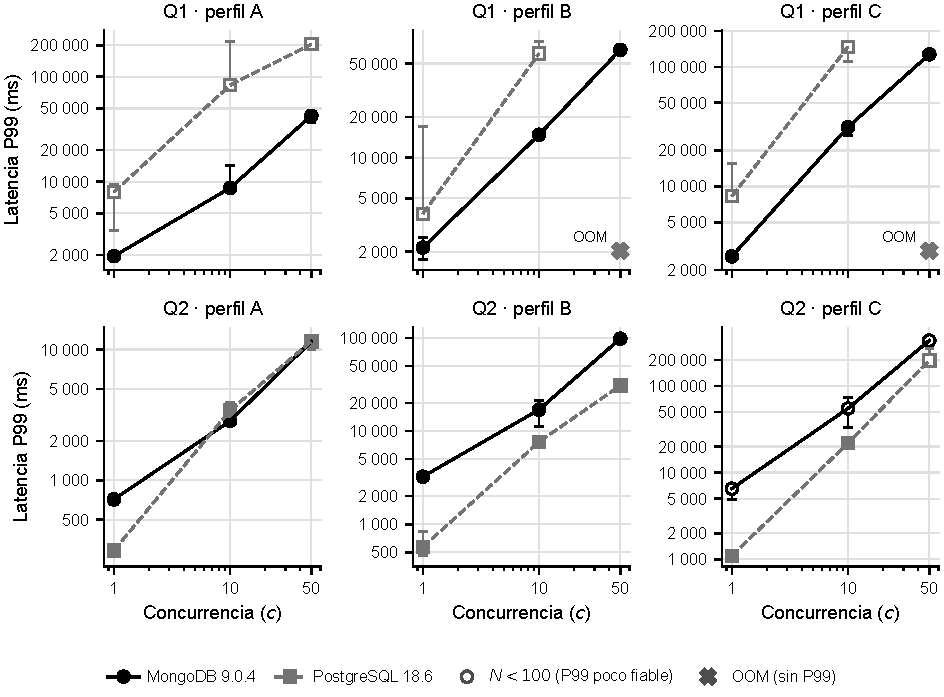
\includegraphics[width=\textwidth]{figures/fig_p99.pdf}
\apanote{Puntos: mediana de tres repeticiones; barras: rango mínimo--máximo. Escala logarítmica en ambos ejes. Marcadores huecos: $N<100$ (P99 poco fiable). Una cruz indica que ninguna consulta se completó por OOM.}
\end{apafig}

\textbf{Limitación de CPU y rendimiento (M1).} En la Figura~\ref{fig:throttle} el tiempo de limitación de CFS en los
perfiles B y C aparece asociado a una caída del rendimiento respecto del perfil A, que permanece cerca de cero segundos. Para \Mongo{} en Q1 con 10 clientes, pasar del perfil A al C redujo el rendimiento un
\fact{dqQ1mCc10}\,\% y aumentó el P99 un \fact{dpQ1mCc10}\,\%; en Q2 la caída fue del \fact{dqQ2mCc10}\,\% y el P99 aumentó un \fact{dpQ2mCc10}\,\%. En \PG{}, Q2 con 10 clientes cayó un
\fact{dqQ2pCc10}\,\% y su P99 aumentó un \fact{dpQ2pCc10}\,\% al pasar de A a C (Tabla~\ref{tab:m1}, Apéndice~A). La limitación depende de cuántos hilos compiten por la cuota: \Mongo{} no registró limitación
en Q1 con 2 CPU y un cliente (\fact{Q1Bc1mthr} s), mientras que \PG{}, que lanza procesos paralelos aun con un cliente, acumuló \fact{Q1Bc1pthr} s en la misma celda.

\begin{apafig}
\caption{Relación entre el tiempo de limitación de CFS y el rendimiento}\label{fig:throttle}
\centering
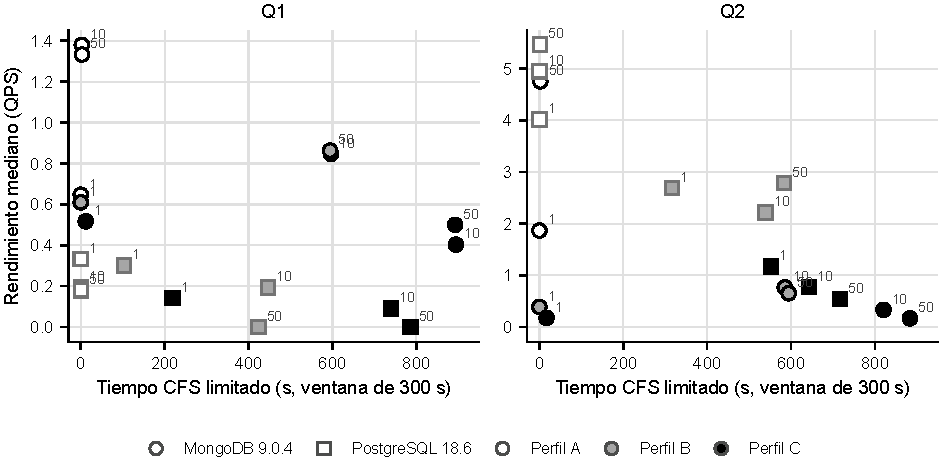
\includegraphics[width=\textwidth]{figures/fig_throttle.pdf}
\apanote{Cada punto es una celda (mediana de tres repeticiones); la etiqueta es la concurrencia $c$. El tiempo se acumula por cola de ejecución del conjunto de CPU, por lo que puede superar los 300 s de la ventana.}
\end{apafig}

\textbf{Memoria en el tiempo (M2/M3).} La Figura~\ref{fig:memory} contrasta tres corridas del perfil C. \Mongo{} estabiliza su memoria de motor en torno a 400 MiB,
muy por debajo del límite. \PG{} con un cliente crece de 120 a unos 330 MiB conforme se llenan
los \textit{shared buffers}, y la caché de páginas oscila hasta el límite por la escritura y lectura de archivos temporales. Con 50 clientes, la memoria del motor
llega al techo de 1\,024 MiB de forma repetida, y cada caída es consistente con la terminación de procesos de usuario por el kernel.

\begin{apafig}
\caption{Memoria del cgroup durante corridas representativas del perfil C}\label{fig:memory}
\centering
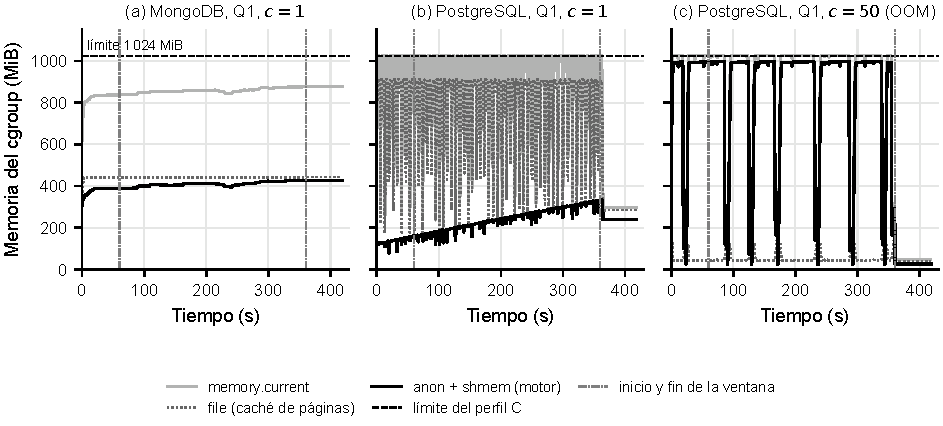
\includegraphics[width=\textwidth]{figures/fig_memory.pdf}
\apanote{Corridas \code{mongodb-C-Q1-c1-r1}, \code{postgresql-C-Q1-c1-r1} y \code{postgresql-C-Q1-c50-r1}. El tiempo parte del inicio del calentamiento; las líneas verticales delimitan la ventana de medición.}
\end{apafig}

\subsection{Planes de ejecución}
La Tabla~\ref{tab:planes} resume los planes capturados fuera de la ventana medida con \code{EXPLAIN (ANALYZE, BUFFERS, VERBOSE)} en
\PG{} y \code{explain("executionStats")} en \Mongo{}; sirven para comparar la forma de los planes, no las magnitudes de latencia, porque son ejecuciones individuales.

\begin{apatab}
\caption{Resumen de los planes de ejecución de Q1 y Q2 (variante estricta)}\label{tab:planes}
\tablefile{tab_plans}
\apanote{Spill: suma de los nodos \textit{Sort} con \textit{external merge} en el plan de \PG{} (MiB). Tiempo: \textit{Execution Time} (\PG{}) o \code{executionTimeMillis} (\Mongo{}).}
\end{apatab}

\textbf{Q1.} \PG{} estima \fact{pgq1estrows} grupos cuando el resultado real es de 96, porque no tiene estadísticas sobre las expresiones aplicadas a los
elementos de \code{jsonb\_array\_elements}. Con esa cardinalidad, descarta una tabla hash y elige \code{GroupAggregate} precedido por un ordenamiento que, en lugar de
operar sobre los elementos desanidados, ordena los documentos completos (ancho de fila de 1\,460 bytes) en cada uno de los tres procesos paralelos: unos \fact{planQ1Cpgdisk} MiB de ordenación
externa por ejecución con \code{work\_mem = 4MB} (Figura~\ref{fig:plan}). \Mongo{} proyecta solo los campos necesarios, desanida y agrupa en una tabla hash que ocupa unos
62 KiB, sin volcar a disco. Con \code{work\_mem = 64MB}, el plan de \PG{} conserva ordenaciones externas por proceso (de unos 226 a 240 MiB), de modo que la variante relajada no elimina el volcado.

\begin{apafig}
\caption{Fragmento del plan de \PG{} para Q1 (perfil C, variante estricta)}\label{fig:plan}
\footnotesize
\setlength{\parindent}{0pt}
{\fontsize{6.5}{7.5}\selectfont\verbatiminput{tables/plan_listing.txt}}
\apanote{Se omitieron costos y líneas intermedias; \texttt{t} es el tiempo real en ms y \texttt{x} el número de iteraciones.}
\end{apafig}

\textbf{Q2.} \PG{} elige un recorrido secuencial paralelo con filtro (\fact{planQ2Apgms} ms en el perfil A y \fact{planQ2Cpgms} ms en el C) seguido de \code{top-N heapsort}
en memoria (unos 276 kB), aunque existe un índice sobre \code{timestamp}: con una selectividad cercana al 45\,\% el planificador prefirió el recorrido secuencial. \Mongo{} usa el índice
\code{timestamp\_1} (\code{IXSCAN} seguido de \code{FETCH}) y examina \fact{planQ2Cmgdocs} documentos y claves antes de ordenar con una cola acotada de 1.35 MB, sin volcado
(\fact{planQ2Amgms} ms en A y \fact{planQ2Cmgms} ms en C). El acceso por índice a casi la mitad de la colección implica lecturas aleatorias de documentos; esto es consistente
con la desventaja de \Mongo{} en los perfiles B y C, que disponen de cachés de WiredTiger de 0.5 y 0.25 GB frente a los 1.5 GB del perfil A. No se recolectaron contadores de la caché de WiredTiger, por lo que esta
explicación no se verificó directamente.

\subsection{Eficiencia de recursos (M3)}
La Figura~\ref{fig:m3} muestra la razón \PG{}/\Mongo{} de la CPU y de la integral de memoria por cada 1\,000 documentos procesados (la Tabla~\ref{tab:m3}, en el Apéndice~B,
contiene los valores absolutos). En Q1, en todas las celdas en que ambos motores terminaron, \PG{} consumió entre \fact{Q1Bc1rcpu} y \fact{Q1Bc10rcpu} veces la CPU de \Mongo{} por cada 1\,000 documentos, y su integral de memoria
fue de \fact{Q1Bc1rmem} a \fact{Q1Ac50rmem} veces la de \Mongo{}. En Q2 la relación se invierte en los perfiles B y C: \PG{} usó entre \fact{Q2Cc1rcpu} y \fact{Q2Cc10rcpu} de la CPU de \Mongo{} (razón PG/Mongo)
y entre \fact{Q2Bc1rmem} y \fact{Q2Cc50rmem} de su integral de memoria; en el perfil A la razón de CPU fue de \fact{Q2Ac50rcpu} a \fact{Q2Ac1rcpu}.

\begin{apafig}
\caption{Razón PostgreSQL/MongoDB del costo de recursos por cada 1\,000 documentos}\label{fig:m3}
\centering
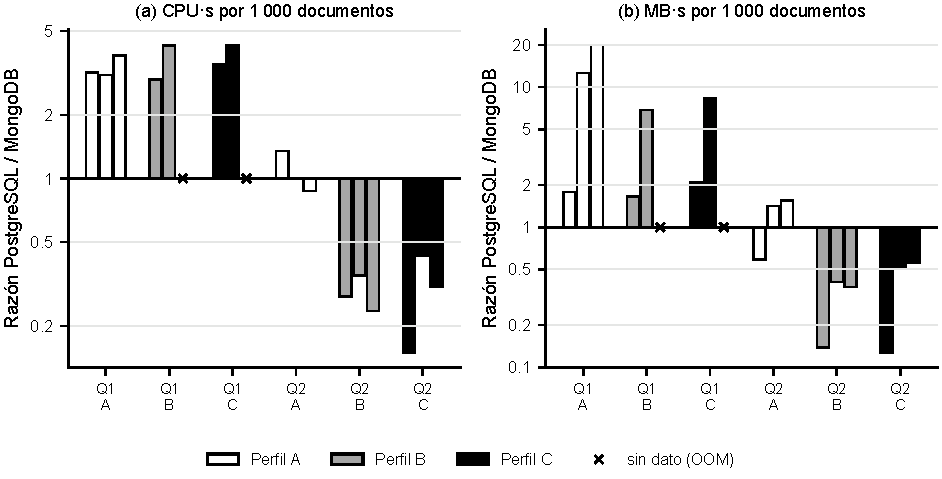
\includegraphics[width=\textwidth]{figures/fig_m3.pdf}
\apanote{Las barras parten de 1 (paridad): hacia arriba, \PG{} consume más; hacia abajo, menos. Tres barras por grupo: $c=1$, 10 y 50. Una cruz indica ausencia de dato por OOM.}
\end{apafig}

\subsection{Contraste de memoria estricta y relajada}
La Tabla~\ref{tab:relajada} compara ambas variantes. En Q1 del perfil C con un cliente, la variante relajada aumentó el rendimiento de \PG{} en un factor de \fact{relqQ1pCc1} (QPS relajado/estricto) y redujo el P99 un
27\,\% (razón \fact{relQ1pCc1}), pero con 10 clientes pasó de \textit{spill} a OOM y con 50 ambas variantes terminan en OOM. En Q2, cuya ordenación acotada no excede los límites de memoria, la razón P99 relajada/estricta
osciló entre \fact{relq2min} y \fact{relq2max} (Figura~\ref{fig:relajada}), es decir, sin un efecto atribuible a la variante. Como referencia de ruido, \Mongo{} en Q1 del perfil C, donde \code{allowDiskUse} no interviene porque no hay volcado, varió entre
\fact{relQ1mCc1} y \fact{relQ1mCc50} del P99 estricto, de modo que diferencias de ese orden no deben interpretarse como efecto.

\begin{apatab}
\caption{Contraste entre las variantes estricta y relajada de memoria}\label{tab:relajada}
\tablefile{tab_relaxed}
\apanote{Cada celda muestra estricta / relajada. P99 en ms (mediana de tres repeticiones). Mongo = \Mongo{}; PG = \PG{}. En \PG{}, estricta = \code{work\_mem = 4MB}; relajada = 64 MB.}
\end{apatab}

\begin{apafig}
\caption{Cociente del P99 relajado respecto del estricto en Q2}\label{fig:relajada}
\centering
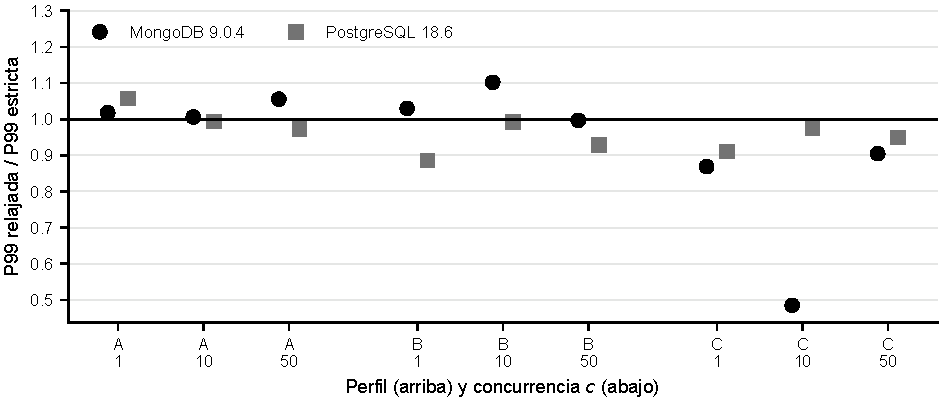
\includegraphics[width=\textwidth]{figures/fig_relaxed.pdf}
\apanote{Un valor de 1 indica ausencia de efecto. Q2 funciona como control negativo: su orden acotado no excede ni el límite de \code{work\_mem} ni el de la etapa de \Mongo{}.}
\end{apafig}

\section{Discusión}
\subsection{Respuesta a las preguntas de investigación}
\textbf{M1 (CPU).} Restringir la CPU degradó a ambos motores, pero de forma desigual según la consulta. La degradación de cola fue mayor en Q2 que en Q1 para \Mongo{}, y mucho mayor para \Mongo{} que para \PG{} en Q2, lo que sugiere que el costo no está solo en la cuota de CPU sino
en cómo accede cada motor a los datos (secuencial frente a aleatorio). La limitación de CFS fue casi nula en el perfil A y de cientos de segundos acumulados en B y C cuando hay varios hilos activos. El paralelismo intra-consulta de \PG{} (dos procesos adicionales por consulta) provoca
limitación incluso con un cliente en los perfiles B y C.

\textbf{M2 (memoria).} Con \code{work\_mem = 4MB}, Q1 obliga a \PG{} a ordenar en disco aproximadamente \fact{planQ1Cpgdisk} MiB por ejecución, mientras que \Mongo{} agrupa en 62 KiB. Cuando el número de sesiones aumenta, la presión se multiplica por proceso y por sesión: con 50 clientes, \PG{} fue terminado por falta de memoria
en los perfiles de 2 y 1 GiB (hasta \fact{oomrssmax} MB de memoria del motor registrados en una corrida OOM) mientras que en el perfil de 4 GiB completó las corridas con volcado. Las 12 corridas OOM sumaron \fact{oomkills} eventos \code{oom\_kill}; en el registro de \PG{} los procesos de usuario
(\textit{backends}) aparecen terminados con la señal 9 mientras el proceso principal sigue operando. Subir \code{work\_mem} a 64 MB no ayudó: con 10 clientes convirtió un volcado tolerable en OOM.

\textbf{M3 (eficiencia).} \Mongo{} requiere entre \fact{Q1Bc1rcpu} y \fact{Q1Bc10rcpu} veces menos CPU por 1\,000 documentos en Q1; en Q2, \PG{} es igual o más eficiente en los perfiles B y C. No hay un motor uniformemente más eficiente: depende de la forma de la consulta.

\subsection{Las seis preguntas del revisor}
La Tabla~\ref{tab:revisor} resume cómo responde este reporte a las seis preguntas de auditoría del \textit{playbook}.
\begin{apatab}
\caption{Respuestas a las seis preguntas del revisor}\label{tab:revisor}
\small
\begin{tabular}{@{}p{0.3in}p{2.1in}p{3.65in}@{}}
\toprule
\# & Pregunta & Evidencia y respuesta \\
\midrule
1 & ¿El baseline es comparable? & Sí. Mismo dataset (semilla 42; SHA-256 del archivo en la sección Método), mismas consultas y mismo recuento y suma en ambos motores tras la carga. \\
2 & ¿P50/P95/P99 con $n$ explícito? & Sí. Tablas~\ref{tab:q1} y~\ref{tab:q2} (columna $N_{\min}$ y marca $^{\dagger}$ para $N<100$). \\
3 & ¿Hubo throttling CFS y cuánto? & Sí. Columna Thr. (delta en la ventana de 300 s); casi nulo en A y de cientos de segundos en B y C (Figura~\ref{fig:throttle}). \\
4 & ¿Spill u OOM, y dónde? & Tabla~\ref{tab:estado}: \PG{} vuelca en toda Q1; OOM en Q1 con $c=50$ en B y C y, en el anexo, con $c=10$ y $50$ en C. \Mongo{} no volcó ni sufrió OOM. \\
5 & ¿Cuántas repeticiones y cómo se resumen? & Tres por celda; mediana y rango $[\min;\max]$ (Tablas~\ref{tab:q1} y~\ref{tab:q2}, Figura~\ref{fig:p99}). \\
6 & ¿El plan respalda el cuello de botella? & Sí. Tabla~\ref{tab:planes} y Figura~\ref{fig:plan}: ordenación externa en Q1 de \PG{}; \textit{top-N heapsort} en Q2; \code{IXSCAN+FETCH} de 226\,680 documentos en \Mongo{}. \\
\bottomrule
\end{tabular}
\end{apatab}

\subsection{Hipótesis}
\textbf{H1} se sostiene: en Q1 \Mongo{} fue más rápido y más eficiente en todas las celdas comparables, y el plan de \PG{} confirma la sobreestimación de grupos y el ordenamiento externo. \textbf{H2} se sostiene con matices: \PG{} fue superior en Q2 a baja concurrencia y bajo restricción de recursos,
pero no hubo diferencia apreciable de rendimiento en el perfil A con 10 o 50 clientes. \textbf{H3} se sostiene parcialmente: con un cliente, la variante relajada mejoró a \PG{} (27\,\% menos P99), y con 10 clientes pasó de volcado a OOM; con 50 clientes la variante estricta ya fallaba, por lo que
no se observa el adelantamiento.

\section{Recomendaciones técnicas para despliegues en la nube}
Las siguientes pautas se derivan de los resultados; las marcadas con asterisco son recomendaciones de buena práctica que esta campaña no evaluó experimentalmente.
\begin{itemize}
\item \textbf{Dimensionar la memoria de \PG{} por sesión y por proceso paralelo, no por consulta aislada.} Con memoria límite y sin \textit{swap}, \code{work\_mem} debe dividirse entre las conexiones activas y los procesos por consulta; en esta campaña, 50 sesiones con 4 MB ya agotaron 1 y 2 GiB en Q1.
\item \textbf{Ajustar el paralelismo a la cuota de CPU.}$^{*}$ \code{max\_parallel\_workers\_per\_gather} debería ser coherente con \code{cpu.max}: con 1 CPU, \PG{} limitó su ejecución durante cientos de segundos acumulados aun con un cliente.
\item \textbf{Evitar agrupar sobre elementos de arreglos JSONB sin estadísticas.} Materializar país y categoría en columnas generadas, o definir estadísticas sobre expresiones,$^{*}$ evita la sobreestimación de \fact{pgq1estrows} grupos y el plan con ordenación externa.
\item \textbf{Fijar \code{wiredTigerCacheSizeGB} explícitamente} en función del límite del contenedor, y vigilar que las consultas con acceso por índice sobre una fracción grande de la colección (como Q2) dispongan de caché suficiente.
\item \textbf{Elegir el motor según el patrón de consulta:} agregaciones con desanidado y agrupación de baja cardinalidad favorecen a \Mongo{}; filtros con orden acotado y recorrido secuencial favorecen a \PG{}, sobre todo con pocos recursos.
\item \textbf{Índices en servicios administrados.} Para indexar \code{(data->{}>'timestamp')::timestamptz} se marcó \code{timestamptz\_in} como \code{IMMUTABLE} en el catálogo, algo imposible sin superusuario en \PG{} administrado; allí debe usarse una función envoltorio \code{IMMUTABLE} propia o extraer la marca de tiempo a una columna nativa.$^{*}$
\end{itemize}

\section{Limitaciones}
\begin{itemize}
\item \textbf{Un solo equipo, virtualizado.} Las corridas usaron Docker Desktop sobre WSL2 en un procesador híbrido de 13.ª generación, no Docker Engine nativo en Linux; los resultados absolutos no son trasladables a servidores y pueden mostrar efectos de la virtualización de E/S.
\item \textbf{Tres repeticiones.} Se reportan medianas y rangos, sin pruebas de significancia. Las razones entre motores son descriptivas.
\item \textbf{P99 con muestras pequeñas.} Todas las celdas de Q1 de \PG{}, las de Q2 de \Mongo{} en el perfil C y la celda de Q2 de \PG{} con 50 clientes en C tienen $N<100$; su P99 es indicativo.
\item \textbf{Intervenciones operativas.} La campaña duró unas \fact{hours} h, con \fact{incidents} incidencias de infraestructura y \fact{discarded} corridas descartadas y repetidas (Apéndice~C): el motor de Docker se degradaba tras 1 a 1.5 h de uso continuo, por lo que se aplicaron reinicios preventivos de Docker Desktop y de WSL2 entre corridas (nunca durante una ventana). El plan se amplió de 144 a 180 corridas y se elevó el límite de incidencias de 4 a 12; ninguno de esos cambios alteró el código de medición.
\item \textbf{Defecto probable en la telemetría.} Parte de los descartes por telemetría (\code{telemetry\_gap}) es compatible con una lectura de \code{/proc/stat} con líneas vacías que interrumpe el muestreador. El archivo está protegido por el manifiesto y no se modificó; cada caso se resolvió repitiendo la corrida.
\item \textbf{Explicaciones no verificadas.} La relación entre el tamaño de la caché de WiredTiger y la lentitud de Q2 en los perfiles B y C es una inferencia a partir del plan de ejecución; no se recolectaron contadores de caché.
\item \textbf{No se midieron} la temperatura ni la frecuencia del procesador durante las 36 h de campaña.
\end{itemize}

\section{Conclusiones}
Bajo límites de recursos de cgroups v2, ningún motor domina de forma general. \Mongo{} resultó más rápido y más eficiente en la agregación con desanidado y no volcó a disco ni sufrió OOM en ninguna de sus 90 corridas, mientras que \PG{} fue superior en la consulta con orden acotado cuando los recursos se reducen. Las consecuencias
prácticas son tres: el costo de una consulta depende del plan y de la forma de acceso a los datos antes que del motor; el límite de memoria sin \textit{swap} convierte los ajustes por sesión en una cuestión de disponibilidad, no solo de rendimiento; y el tiempo de limitación de CFS es una señal de saturación observable que acompaña a
la caída de rendimiento. Como trabajo futuro se propone repetir la matriz en Linux nativo, recolectar contadores de caché de WiredTiger, evaluar estadísticas sobre expresiones y columnas generadas en \PG{} y aumentar el número de repeticiones para sustentar inferencia estadística.

% =============================================================================  REFERENCIAS
\clearpage
\section{Referencias}
\aparef{Cattell, R. (2011). Scalable SQL and NoSQL data stores. \textit{ACM SIGMOD Record, 39}(4), 12--27. \url{https://doi.org/10.1145/1978915.1978919}}
\aparef{Dean, J., \& Barroso, L. A. (2013). The tail at scale. \textit{Communications of the ACM, 56}(2), 74--80. \url{https://doi.org/10.1145/2408776.2408794}}
\aparef{Gregg, B. (2020). \textit{Systems performance: Enterprise and the cloud} (2.\textsuperscript{a} ed.). Addison-Wesley.}
\aparef{Heo, T. (s.\,f.). \textit{Control group v2}. The Linux Kernel documentation. \url{https://docs.kernel.org/admin-guide/cgroup-v2.html}}
\aparef{Hoefler, T., \& Belli, R. (2015). Scientific benchmarking of parallel computing systems: Twelve ways to tell the masses when reporting performance results. En \textit{Proceedings of the International Conference for High Performance Computing, Networking, Storage and Analysis} (Art. 73). ACM. \url{https://doi.org/10.1145/2807591.2807644}}
\aparef{Jain, R. (1991). \textit{The art of computer systems performance analysis: Techniques for experimental design, measurement, simulation, and modeling}. John Wiley \& Sons.}
\aparef{Kleppmann, M. (2017). \textit{Designing data-intensive applications}. O'Reilly Media.}
\aparef{Merkel, D. (2014). Docker: Lightweight Linux containers for consistent development and deployment. \textit{Linux Journal, 2014}(239), Art. 2.}
\aparef{MongoDB, Inc. (s.\,f.). \textit{MongoDB manual}. \url{https://www.mongodb.com/docs/manual/}}
\aparef{Mytkowicz, T., Diwan, A., Hauswirth, M., \& Sweeney, P. F. (2009). Producing wrong data without doing anything obviously wrong! En \textit{Proceedings of the 14th International Conference on Architectural Support for Programming Languages and Operating Systems} (pp. 265--276). ACM. \url{https://doi.org/10.1145/1508244.1508275}}
\aparef{PostgreSQL Global Development Group. (s.\,f.). \textit{PostgreSQL 18 documentation}. \url{https://www.postgresql.org/docs/18/}}
\aparef{Universidad Politécnica de Chiapas. (2026). \textit{Playbook técnico: Medición de métricas en bases documentales} [Documento del curso Bases de Datos en la Nube]. Ingeniería en Tecnologías de la Información e Innovación Digital.}

% =============================================================================  APÉNDICES
\clearpage
\FloatBarrier
\section{\texorpdfstring{Apéndice A\\Variación por contención de CPU (M1)}{Apéndice A. Variación por contención de CPU (M1)}}
{\footnotesize\singlespacing
\setlength{\tabcolsep}{3pt}
\begin{longtable}{@{}lllllrrrrrr@{}}
\caption{Variación del rendimiento y del P99 de los perfiles B y C respecto del perfil A}\label{tab:m1}\\
\toprule
Q & Motor & $c$ & Perf. & QPS A & QPS & $\Delta$QPS & P99 A & P99 & $\Delta$P99 & Thr. (s) \\
\midrule\endfirsthead
\toprule
Q & Motor & $c$ & Perf. & QPS A & QPS & $\Delta$QPS & P99 A & P99 & $\Delta$P99 & Thr. (s) \\
\midrule\endhead
\bottomrule\endlastfoot
Q1 & Mongo & 1 & B & 0.647 & 0.610 & -6\% & 1\,949 & 2\,149 & +10\% & 0.0 \\
Q1 & Mongo & 1 & C & 0.647 & 0.517 & -20\% & 1\,949 & 2\,598 & +33\% & 11.6 \\
Q1 & Mongo & 10 & B & 1.380 & 0.847 & -39\% & 8\,723 & 14\,802 & +70\% & 596.8 \\
Q1 & Mongo & 10 & C & 1.380 & 0.403 & -71\% & 8\,723 & 31\,353 & +259\% & 894.4 \\
Q1 & Mongo & 50 & B & 1.333 & 0.863 & -35\% & 42\,502 & 63\,186 & +49\% & 594.6 \\
Q1 & Mongo & 50 & C & 1.333 & 0.500 & -62\% & 42\,502 & 127\,111 & +199\% & 892.7 \\
Q1 & PG & 1 & B & 0.333 & 0.300 & -10\% & 7\,967 & 3\,822 & -52\% & 102.8 \\
Q1 & PG & 1 & C & 0.333 & 0.143 & -57\% & 7\,967 & 8\,279 & +4\% & 218.8 \\
Q1 & PG & 10 & B & 0.193 & 0.193 & +0\% & 83\,191 & 59\,291 & -29\% & 446.3 \\
Q1 & PG & 10 & C & 0.193 & 0.090 & -53\% & 83\,191 & 146\,758 & +76\% & 739.6 \\
Q1 & PG & 50 & B & 0.180 & 0.000 & -100\% & 204\,550 & --- & --- & 424.1 \\
Q1 & PG & 50 & C & 0.180 & 0.000 & -100\% & 204\,550 & --- & --- & 786.5 \\
\addlinespace[2pt]
Q2 & Mongo & 1 & B & 1.867 & 0.390 & -79\% & 715 & 3\,239 & +353\% & 0.0 \\
Q2 & Mongo & 1 & C & 1.867 & 0.177 & -91\% & 715 & 6\,530 & +813\% & 17.0 \\
Q2 & Mongo & 10 & B & 4.943 & 0.767 & -84\% & 2\,844 & 16\,982 & +497\% & 585.1 \\
Q2 & Mongo & 10 & C & 4.943 & 0.333 & -93\% & 2\,844 & 55\,053 & +1836\% & 820.6 \\
Q2 & Mongo & 50 & B & 4.753 & 0.653 & -86\% & 11\,526 & 98\,309 & +753\% & 594.4 \\
Q2 & Mongo & 50 & C & 4.753 & 0.167 & -96\% & 11\,526 & 334\,436 & +2802\% & 883.5 \\
Q2 & PG & 1 & B & 4.013 & 2.693 & -33\% & 291 & 567 & +95\% & 316.4 \\
Q2 & PG & 1 & C & 4.013 & 1.177 & -71\% & 291 & 1\,093 & +276\% & 552.2 \\
Q2 & PG & 10 & B & 4.950 & 2.217 & -55\% & 3\,420 & 7\,657 & +124\% & 539.6 \\
Q2 & PG & 10 & C & 4.950 & 0.773 & -84\% & 3\,420 & 21\,961 & +542\% & 643.0 \\
Q2 & PG & 50 & B & 5.467 & 2.787 & -49\% & 11\,552 & 30\,744 & +166\% & 582.9 \\
Q2 & PG & 50 & C & 5.467 & 0.543 & -90\% & 11\,552 & 196\,714 & +1603\% & 716.5 \\
\end{longtable}
}
\par\vspace{3pt}{\footnotesize\noindent\textit{Nota.} QPS A y P99 A son los valores del perfil A; $\Delta$ = variación porcentual respecto de A; P99 en ms; Thr. = tiempo de limitación de CFS (s). Mongo = \Mongo{}; PG = \PG{}. Celdas sin dato: OOM.\par}

\clearpage
\section{\texorpdfstring{Apéndice B\\Eficiencia de recursos por cada 1\,000 documentos (M3)}{Apéndice B. Eficiencia de recursos por cada 1000 documentos (M3)}}
{\footnotesize\singlespacing
\setlength{\tabcolsep}{3pt}
\begin{longtable}{@{}lllrrrrrrrr@{}}
\caption{CPU, pico e integral de memoria por cada 1\,000 documentos procesados}\label{tab:m3}\\
\toprule
Q & Perf. & $c$ & CPU Mongo & CPU PG & PG/Mongo & Pico Mongo & Pico PG & Int. Mongo & Int. PG & PG/Mongo \\
\midrule\endfirsthead
\toprule
Q & Perf. & $c$ & CPU Mongo & CPU PG & PG/Mongo & Pico Mongo & Pico PG & Int. Mongo & Int. PG & PG/Mongo \\
\midrule\endhead
\bottomrule\endlastfoot
Q1 & A & 1 & 0.0031 & 0.0099 & 3.2 & 681 & 930 & 2.10 & 3.74 & 1.8 \\
Q1 & A & 10 & 0.0058 & 0.0178 & 3.1 & 738 & 1\,394 & 1.08 & 13.52 & 12.6 \\
Q1 & A & 50 & 0.0060 & 0.0229 & 3.8 & 922 & 2\,640 & 1.38 & 27.57 & 20.0 \\
Q1 & B & 1 & 0.0033 & 0.0098 & 2.9 & 663 & 651 & 2.08 & 3.44 & 1.7 \\
Q1 & B & 10 & 0.0047 & 0.0201 & 4.3 & 715 & 1\,130 & 1.64 & 11.29 & 6.9 \\
Q1 & B & 50 & 0.0046 & --- & --- & 805 & 1\,991 & 1.82 & --- & --- \\
Q1 & C & 1 & 0.0039 & 0.0134 & 3.5 & 427 & 330 & 1.59 & 3.34 & 2.1 \\
Q1 & C & 10 & 0.0050 & 0.0213 & 4.3 & 453 & 856 & 2.19 & 18.14 & 8.3 \\
Q1 & C & 50 & 0.0040 & --- & --- & 607 & 997 & 2.33 & --- & --- \\
\addlinespace[2pt]
Q2 & A & 1 & 0.0011 & 0.0014 & 1.3 & 687 & 864 & 0.73 & 0.43 & 0.6 \\
Q2 & A & 10 & 0.0016 & 0.0016 & 1.0 & 713 & 1\,009 & 0.29 & 0.41 & 1.4 \\
Q2 & A & 50 & 0.0017 & 0.0015 & 0.9 & 803 & 1\,434 & 0.34 & 0.52 & 1.5 \\
Q2 & B & 1 & 0.0054 & 0.0015 & 0.3 & 624 & 582 & 3.12 & 0.43 & 0.1 \\
Q2 & B & 10 & 0.0052 & 0.0018 & 0.3 & 623 & 727 & 1.61 & 0.65 & 0.4 \\
Q2 & B & 50 & 0.0061 & 0.0014 & 0.2 & 721 & 1\,148 & 2.19 & 0.82 & 0.4 \\
Q2 & C & 1 & 0.0113 & 0.0017 & 0.1 & 387 & 313 & 4.15 & 0.53 & 0.1 \\
Q2 & C & 10 & 0.0060 & 0.0026 & 0.4 & 387 & 458 & 2.30 & 1.17 & 0.5 \\
Q2 & C & 50 & 0.0120 & 0.0037 & 0.3 & 479 & 871 & 5.75 & 3.18 & 0.6 \\
\end{longtable}
}
\par\vspace{3pt}{\footnotesize\noindent\textit{Nota.} CPU en CPU$\cdot$s por 1\,000 documentos; Pico = máximo de \code{anon}$+$\code{shmem} (MB); Int. = integral de memoria (MB$\cdot$s por 1\,000 documentos). PG/Mongo = razón entre ambos motores.\par}

\clearpage
\section{\texorpdfstring{Apéndice C\\Intervenciones operativas durante la campaña}{Apéndice C. Intervenciones operativas durante la campaña}}
\begin{apatab}
\caption{Registro resumido de intervenciones operativas}\label{tab:interv}
\small
\begin{tabular}{@{}p{1.8in}p{1.4in}p{2.8in}@{}}
\toprule
Intervención & Fecha y hora & Detalle \\
\midrule
Ampliación del plan & 31 oct., 10:30 & De 144 a 180 corridas; las 36 nuevas (Q2 relajada en A y B) se añadieron al final. \\
Límite de incidencias & 31 oct., 12:44 & \code{MAX\_INCIDENTS} de 4 a 12 (archivo no protegido). \\
Paradas por presupuesto de incidencias & 31 oct., 04:35--09:35 y 11:04--12:39 & Corridas de \Mongo{} y de \PG{} descartadas repetidamente por fallos de telemetría; reanudación tras reiniciar Docker. \\
Apagado accidental del equipo & 31 oct., 12:35 & Sin corrida en curso (campaña ya detenida); datos íntegros. \\
Motor de Docker bloqueado & 31 oct., 18:22--21:57 & Reinicio fallido en dos ocasiones; resuelto con un reinicio limpio de Docker Desktop. \\
Reinicios preventivos de Docker y WSL2 & 31 oct., 14:25 a 1 nov., 13:36 & 16 ciclos de pausa limpia, reinicio, comprobación y reanudación; sin pérdida de corridas registradas. \\
Corridas descartadas & Toda la campaña & \fact{discarded} intentos repetidos desde cero (telemetría, arranque de procesos cliente, orquestación). \\
\bottomrule
\end{tabular}
\apanote{El registro detallado, con hora y motivo de cada intervención, se conserva en \code{docs/bitacora\_supervision.md}. La supervisión operativa se apoyó en un asistente automatizado.}
\end{apatab}

\clearpage
\section{\texorpdfstring{Apéndice D\\Reproducibilidad}{Apéndice D. Reproducibilidad}}
\noindent Los artefactos de la campaña (código, consultas, perfiles, CSV, series de 1\,Hz y planes de ejecución) están en el repositorio del proyecto. Las figuras y tablas de este reporte se regeneran con
\code{report/src/build_assets.py} a partir de \code{results/mediciones.csv}, \code{results/anexo\_variantes.csv}, \code{results/raw/} y \code{results/explain/}.
Imágenes fijadas por \textit{digest}: \code{mongo:9.0.4@sha256:452bdaf2\ldots a058}; \code{postgres:18.6@sha256:979bccfd\ldots 0e4}; \code{cadvisor v0.60.6@sha256:b8e7d109\ldots d1bd07a};
\code{prometheus v3.15.1@sha256:fa330227\ldots f191a2}; \code{node-exporter v1.12.1@sha256:1b4e4438\ldots 1f1be0}. Los \textit{digests} completos están en \code{docker-compose.yml}.

\end{document}
